\item[6.~定理.] \emph{三角形の各辺の中点に立てた垂線は、そのうち二本が平行ならば、すべて平行である。}

\begin{figure}[h]
\centering
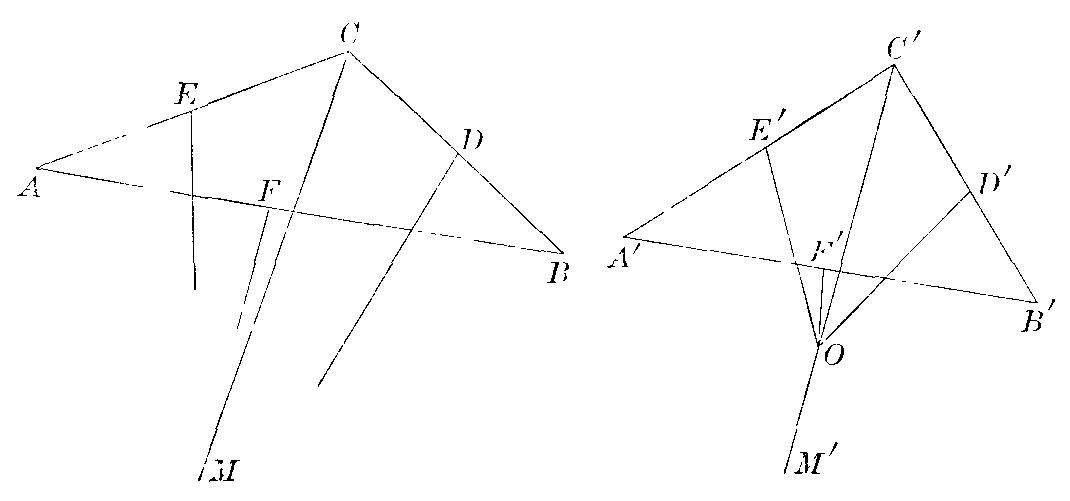
\includegraphics[width=90mm]{fig40.png}
\end{figure}

\textbf{$A$}、$B$、$C$ を三角形の頂点とし、$D$、$E$、$F$ をそれぞれの対辺の中点とする。$D$ と $E$ での垂線が平行であると与えられているとき、$F$ での垂線もそれらに平行であることを証明する。

\textbf{証明.} 与えられた二本の平行な垂線に平行に、$C$ を通る $CM$ を引く。$CM$ は、$C$ の二辺とのあいだに平行角 $\Pi\left(\dfrac{a}{2}\right)$ と $\Pi\left(\dfrac{b}{2}\right)$ をなし、$C$ での角はこれらの和または差である。和になるのは $C$ が与えられた垂線の間にあるとき、差になるのは $C$ が両方の同じ側にあるときである。$CA$ と $CB$ の長さを変えずに、$C$ でのこれらの角を適当に小さくすることによって、それらの中点 $D$ と $E$ での垂線が、$C$ から $\frac{a}{2}$ より大きく、かつ $\frac{b}{2}$ より大きい任意の距離のところで、$CM$ と、したがって互いに、交わるようにできる。

こうしてできた三角形を $A'B'C'$ とし、与えられた二本の垂線が交わる点を $O$、$O$ を通る線を $C'M'$ とする。三角形 $A'B'C'$ では、三本の垂線は点 $O$ で交わる（第I章, I, 5）。さて、作図をそのままにして、$O$ を $C'M'$ 上で遠ざけることができる。すなわち、線 $C'A'$ と $C'B'$ を、長さを変えずに $C'$ のまわりに回転させ、三本の垂線 $D'O$、$E'O$、$F'O$ がつねに $O$ を通るようにする。$O$ が限りなく遠ざかるとき、$C'$ での角は極限として $\Pi\left(\dfrac{a}{2}\right)$ と $\Pi\left(\dfrac{b}{2}\right)$ に近づき、三本の垂線は、$C'M'$ に、また互いに、平行な位置に近づく。しかし三角形 $A'B'C'$ は、極限として、二辺とその間の角がそれぞれ $ABC$ の対応する部分に等しい三角形、すなわち $ABC$ に等しい三角形に近づく。ゆえに $ABC$ では、三本の垂線はすべて平行である。

\item[7.~定理.] \emph{交わらず、平行でもない二直線は、ただ一つの共通垂線をもつ。}

\textbf{証明.} $AB$ と $CD$ をその二直線とし、$AB$ の任意の点 $A$ から $CD$ に垂線 $AC$ を下ろす。$AC$ 自身が共通垂線でなければ、$AC$ が $AB$ となす角の一方は鋭角である。この角が $AB$ の側にあるとして、$BAC < \frac{\pi}{2}$ とする。$AC$ の同じ側に、$CD$ に平行に $AE$ を引く。$AB$ は $CD$ に平行でもなく交わりもしないから、角 $EAC$ は $BAC$ より小さい。角 $EAC$ の内部に任意の線 $AH$ を引き、$CD$ と $H$ で交わらせる。$H$ が $C$ の位置から出発して線 $CD$ 上を限りなく遠ざかるならば、角 $BAH$ は角 $BAC$ の大きさから角 $BAE$ まで減少する。角 $AHC$ は、$BAC$ より大きい直角である $C$ での角の大きさから、\emph{限りなく}減少する。したがって $BAH=AHC$ となる位置がある。この位置では、$AH$ の中点を通って与えられた二直線の一方に垂直な線 $NM$ は、第I章, I, 10 で証明したように、他方にも垂直である。

\begin{figure}[h]
\centering
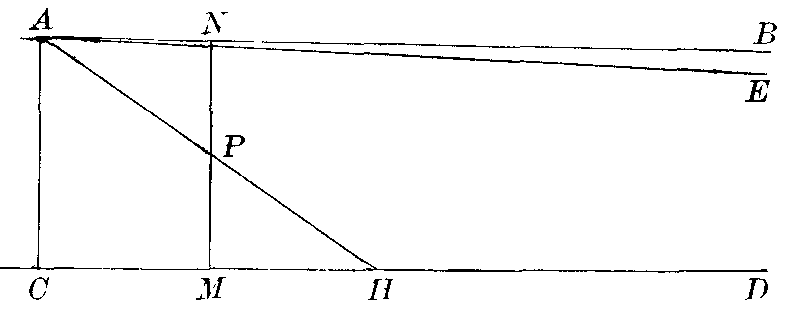
\includegraphics[width=80mm]{fig41.png}
\end{figure}

共通垂線が二本あれば長方形ができるが、それは双曲幾何学では不可能である。

\item[8.~定理.] \emph{三角形の各辺の中点に立てた垂線が、交わらず、平行でもないならば、それらはすべてある直線に垂直である。}

\begin{figure}[h]
\centering
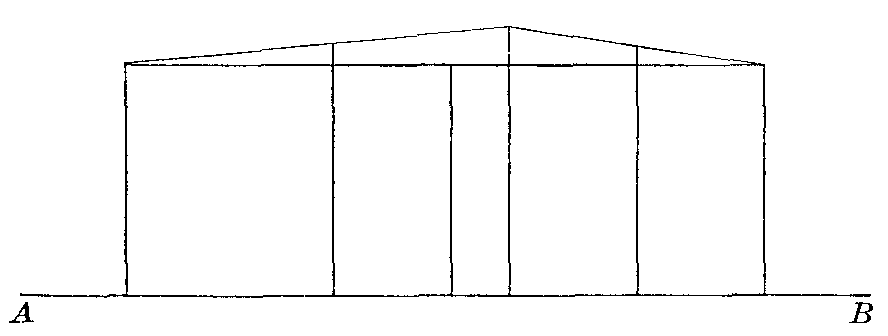
\includegraphics[width=90mm]{fig42.png}
\end{figure}

\textbf{証明.} これらの線のうち二本に垂直な線 $AB$ を引くことができ、第I章, II, 13 により、三角形の三つの頂点からこの線へ下ろした垂線は等しい。これら三つのうちの任意の二つの中間に立てた $AB$ への垂線は、三角形の対応する辺に対して、その中点で垂直である（第I章, I, 11）。こうして、三角形の各辺の中点に立てた三本の垂線はすべて $AB$ に垂直である。

直線は、平面への射影に平行であるとき、その平面に平行であるという。

\item[9.~定理.] \emph{平面にない任意の直線に対して、平面に垂直で、その直線に平行な線を引くことができる。}

\begin{figure}[h]
\centering
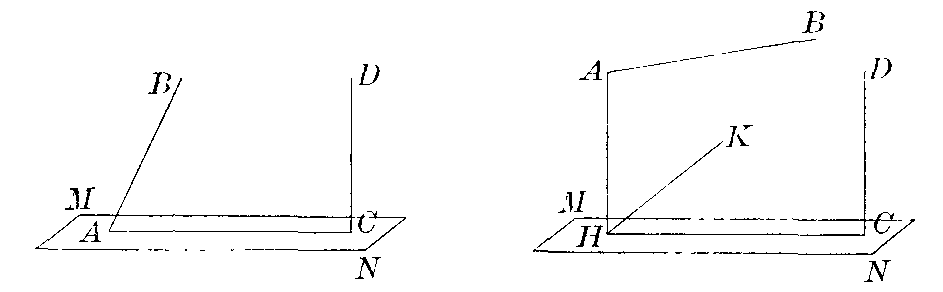
\includegraphics[width=100mm]{fig43.png}
\end{figure}

\textbf{証明.} $AB$ を与えられた直線、$MN$ を平面とする。$AB$ が平面 $MN$ と点 $A$ で出会うならば、その射影上に、$A$ での角が $\Pi(AC)$ に等しくなるような長さ $AC$ をとる。すると、$C$ で平面に垂直な $CD$ は $AB$ に平行になる。同様にして、平面の反対側にも、延長した $BA$ に平行な垂線を引くことができる。

$AB$ が $MN$ と出会わないならば、少なくとも一方の向きでは $MN$ から離れてゆく。平面上の $AB$ の射影の任意の点 $H$ を通って、$MN$ から離れてゆく $AB$ の部分に向かって、$AB$ に平行な線 $HK$ を引き、つぎにこの線に平行で平面に垂直な $CD$ を引くことができる。

$AB$ が $MN$ に平行でなければ、それは平面とどこかの点で出会うか、平面と線が共通垂線をもち、線が両方の向きで平面から離れてゆくかのいずれかである。後者の場合には、線に平行な垂線が二本あり、線の各部分に対して一本ずつ平行である。

二本の垂線が、線の同じ向きに対して平行であることはできない。そうなれば、それらは互いに平行になるが、平面に垂直で互いに平行な二直線は存在しないからである。
\end{description}

\section{限界曲線と限界面、等距離曲線と等距離面}

直線 $AB$ が与えられたとき、その端点 $A$ で任意の角をとり、辺 $AC$ を、その中点に立てた垂線が $AB$ に平行になるように延長する。点 $C$ の軌跡は、\emph{オリサイクル}あるいは\emph{限界曲線}と呼ばれる曲線である。$AB$ はその\emph{軸}である。

\begin{figure}[h]
\centering
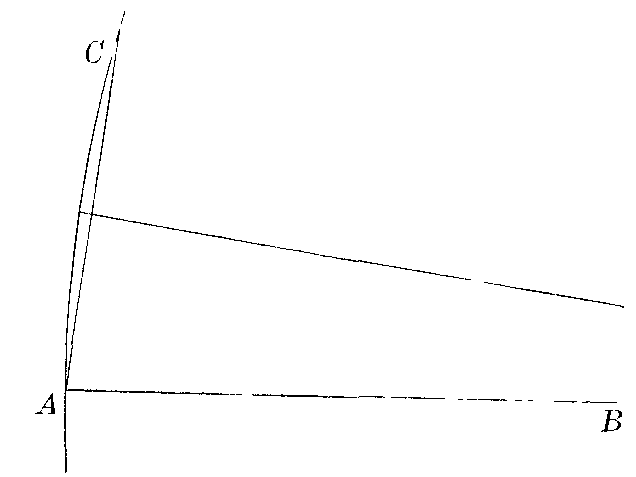
\includegraphics[width=60mm]{fig44.png}
\end{figure}

定義から、すべての限界曲線は等しく、限界曲線はその軸に関して対称である。すなわち、その軸のまわりに二直角だけ回転させると、それ自身に重なる。

\begin{description}
\item[1.~定理.] \emph{限界曲線の軸に平行な任意の線を軸にとることができる。}

\textbf{$AB$} を軸、$CD$ を $AB$ に平行な任意の線とし、$CD$ を軸にとれることを証明する。

\begin{figure}[h]
\centering
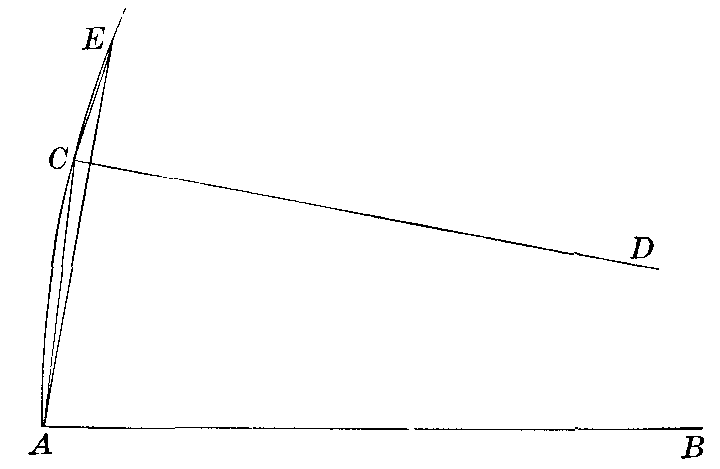
\includegraphics[width=70mm]{fig45.png}
\end{figure}

\textbf{証明.} $AC$ を引く。また、曲線上の任意の他の点 $E$ に、$AE$ と $CE$ を引く。$AC$ の中点と $AE$ の中点に立てた垂線は、$AB$ と $CD$ に、また互いに平行である。したがって、三角形 $ACE$ の第三辺 $CE$ の中点に立てた垂線は、それらに、また $CD$ に平行である。ゆえに $CD$ を軸にとることができる。

\textbf{系.} \emph{限界曲線は、形を変えずにそれ自身の上を滑らせることができる。すなわち、曲率が一定である。}

\item[2.~定理.] \emph{共通の軸の組をもつ二つの限界曲線は、軸のそれぞれの上に同じ距離を切り取り、対応する弧の比はこの距離だけに依存する。}

\begin{figure}[h]
\centering
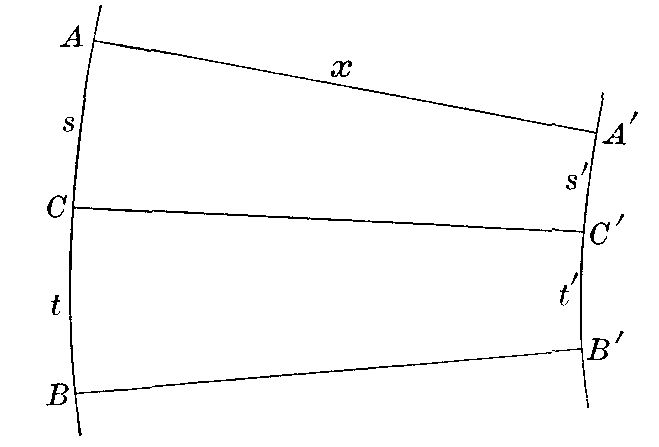
\includegraphics[width=70mm]{fig46.png}
\end{figure}

\textbf{証明.} 任意の二つの軸をとり、第三の軸が、最初の二つが二つの限界曲線の一方の上に切り取る弧を二等分するようにとる。図形をこの軸のまわりに回転させることによって、曲線が二つの軸の上に等しい距離を切り取ることが示される。

$AA'$、$BB'$、$CC'$ を、二つの限界曲線 $AB$ と $A'B'$ の任意の三つの軸とし、それらの共通の長さを $x$ とし、それらが $AB$ 上に弧 $s$ と $t$ を、$A'B'$ 上に $s'$ と $t'$ を切り取るとする。

$s = t$ のとき $s' = t'$ であり、一般に、
\begin{equation*}
\frac{s}{t} = \frac{s'}{t'}
\end{equation*}
である。これは、まず $s$ と $t$ が通約できるときに証明し、ついで通約できないときには極限の方法によって証明する。したがって比 $\frac{s}{s'}$ は、与えられた $x$ の値に対して定数である。

$\dfrac{s}{s'} = f(x)$ とおく。

\begin{figure}[h]
\centering
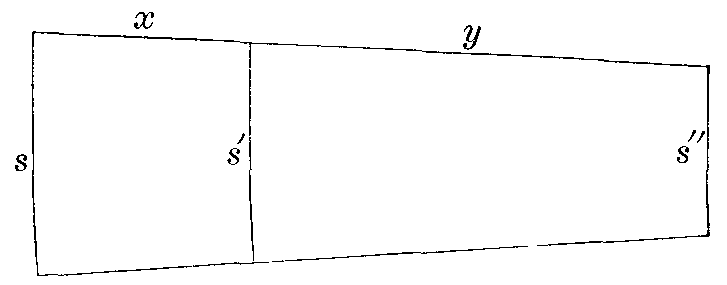
\includegraphics[width=70mm]{fig47.png}
\end{figure}

同じ軸の組をもつ三つの限界曲線から、
\begin{equation*}
f(x+y) = f(x)f(y)
\end{equation*}
を得る。この性質は指数関数に特有のもので、その一般形は $f(x)= e^{ax}$ である。\footnote{$y = x$、$2x$、$\cdots$ $(n-1)x$ を順次代入すると、$x$ を任意の正の量として、正の整数値 $n$ に対して
\begin{equation*}
f(nx) = [f(x)]^n
\end{equation*}
を得る。
\par ところで、
\begin{equation*}
f\left(\frac{r}{s}x\right) = \left[f\left(\frac{x}{s}\right)\right]^r
\end{equation*}
であり、これは等式
\begin{equation*}
\left[f\left(\frac{x}{s}\right)\right]^s = f(x)
\end{equation*}
の左辺の $s$ 乗根の $r$ 乗である。したがって、
\begin{equation*}
f\left(\frac{r}{s}x\right) = [f(x)]^\frac{r}{s}.
\end{equation*}
こうして、$f(x)$ が $x$ の連続関数であると仮定すれば、$x$ と $n$ のすべての実数の正の値に対して
\begin{gather*}
f(nx) = [f(x)]^n, \\
\intertext{が証明され、$n$ に $x$ を、$x$ に $1$ を代入すれば、}
f(x) = [f(1)]^x
\end{gather*}
を得る。
\par $f(1) = e^a$ と書くと、
\begin{equation*}
f(x) = e^{ax}
\end{equation*}
となる。} したがって、$\dfrac{s}{s'}= e^{ax}$ であり、$a$ の値は測定の単位に依存する（後述の該当ページを見よ）。

\item[3.~定理.] \emph{同じ軸をもつ二つの限界曲線と、それらの共通な二つの軸とで囲まれた面積は、切り取られた弧の差に比例する。}

\begin{figure}[h]
\centering
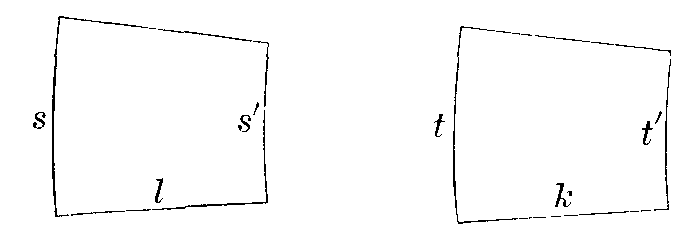
\includegraphics[width=60mm]{fig48.png}
\end{figure}

\textbf{証明.} $s$ と $s'$ を切り取られた弧の長さ、$l$ を軸上で測った、それらの間の距離とする。同様にしてつくった第二の図形について、対応する量を $t$、$t'$、$k$ とする。

二つの図形の対応する線がすべて等しければ、重ね合わせることができるから、面積は等しい。$k = l$ だけが成り立つならば、面積は対応する弧、たとえば $s' : t'$ の比になる。これは、まず弧が通約できる場合に証明し、ついで通約できない場合には極限の方法によって証明する。

\begin{figure}[h]
\centering
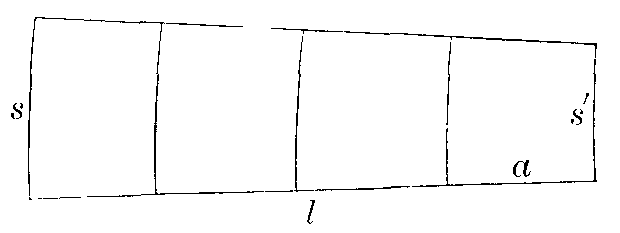
\includegraphics[width=60mm]{fig49.png}
\end{figure}

$l$ と $k$ が通約できるとき、
\begin{equation*}
\frac{l}{m} = \frac{k}{n} = a
\end{equation*}
とする。軸上に、$a$ に等しい距離ごとに一連の限界曲線を引き、面積をそれぞれ $m$ 個と $n$ 個の部分に分けることができる。距離 $a$ に対応する弧の比を $r$ とすれば、これらの部分は、次の量に比例する。
\begin{gather*}
  s',\ s'r,\ s'r^2,\dots s'r^{m-1};\\
  t',\ t'r,\ t'r^2,\dots t'r^{n-1}.
\end{gather*}

したがって二つの面積の比は、
\begin{equation*}
  s' \frac{r^m-1}{r-1} \colon t' \frac{r^n-1}{r-1}
\end{equation*}
である。

しかるに、
\begin{equation*}
  s'r^m = s \text{ かつ } t'r^n = t
\end{equation*}
であるから、これは比
\begin{equation*}
  s-s' \colon t-t'
\end{equation*}
と同じである。

$l$ と $k$ が通約できないときは、他の同様な証明のように進める。

この定理は、多角形について証明した定理と類似している。すなわち、面積は、図形を一周するときの、四直角を超える回転量に比例し、限界曲線に沿って進むときの回転の割合は一定だからである。

\begin{figure}[h]
\centering
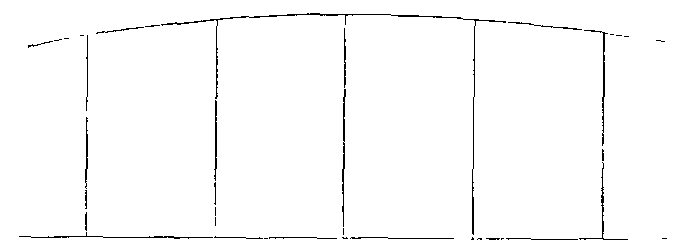
\includegraphics[width=60mm]{fig50.png}
\end{figure}

直線から与えられた距離にある点の軌跡は、\emph{等距離曲線}と呼ぶことのできる曲線である。この曲線の異なる点から基線へ下ろした垂線は等しく、曲線の\emph{軸}と呼ぶことができる。

等距離曲線は、その軸の一つのまわりに二直角だけ回転させたとき、あるいはそれ自身の上を滑らせたとき、それ自身に重なる。曲率は一定である。

同じ軸の組をもつ二つの限界曲線の場合とまったく同様に、等距離曲線上の弧は、その軸が基線上に、あるいは同じ軸の組をもつ他の任意の等距離曲線上に、端点で切り取る線分に比例することを証明できる。

